

\question(20分){已知控制系统结构图如下所示,已知 $G(s)=\frac{1}{s+1},G_c(s)=1$ 。 若 $G_r(s)=\frac{k_1 s+k_2}{s+1},r(t)=t,(t>0)$ , 分析是否存在 $k_1,k_2$ 使稳态误差为零。


\begin{tikzpicture}[node distance=3em,auto,>=latex', thick]
%\path[use as bounding box] (-1,0) rectangle (10,-2); 
\tikzstyle{block} = [draw,rectangle,thick,minimum height=1em,minimum width=1em]
\tikzstyle{sum} = [draw,circle,inner sep=0mm,minimum size=2mm]
\tikzstyle{branch} = [circle,fill,inner sep=0pt,minimum size=1mm]
\tikzstyle{connector} = [->,thick]

\def\r{\node(r){$r(t)$};}
\def\b(#1){\node[branch](b#1){};}
\def\p(#1){\node[sum](p#1){};}
\def\gc{\node[block](gc){$G_c(s)$};}
\def\gr{\node[block](gr){$G_r(s)$};}
\def\gp{\node[block](gp){$G(s)$};}
\def\g(#1){\node[block](g#1){$1$};}
\def\c{\node(c){$c(t)$};}

\matrix[ampersand replacement=\&, row sep=1em, column sep=2em]{
	\&         \&   \gr  \\
	\r  \&   \b(r)  \& \p(e)  \& \gc \& \p(r) \& \gp \& \b(c)  \& \c  \\
	\&         \&         \& \g(h)    \\
};
\draw [connector](r) -- (pe) ; 
\draw [connector](br) |- (gr) ; 
\draw [connector](gr) -| (pr) ; 
\draw [connector](pe) -- node[midway]{$E(s)$} (gc) ; 
\draw [connector](gc) -- (pr) ; 
\draw [connector](pr) -- (gp) ; 
\draw [connector](gp) -- (c) ; 
\draw [connector](bc) |- (gh) ; 
\draw [connector](gh) -| node[near end , left]{$-$} (pe) ; 
\end{tikzpicture} 

\onlyanswer
{
	答:当 $G_r(s)=\frac{k_1 s+k_2}{s+1},r(t)=t,(t>0)$ 时,得:
	\begin{align*}
	\frac{E(s)}{R(s)} &= (1-\frac{k_1s+k_2}{s+1}\cdot\frac{1}{s+1})\frac{1}{1+\frac{1}{s+1}} \\
	&=\frac{(s+1)^2-(k_1s+k_2)}{(s+2)(s+1)} \\
	&=\frac{s^2+(2-k_1)s+(1-k_2)}{(s+2)(s+1)} \\
	\end{align*}
	所以,当 $k_1=2,k_2=1$ 时,
	\begin{align*}
	E(s) &=\frac{s^2+(2-k_1)s+(1-k_2)}{(s+2)(s+1)}\cdot R(s) \\
	&=\frac{s^2}{(s+2)(s+1)}\cdot \frac{1}{s^2} \\
	&=\frac{1}{(s+2)(s+1)} \\
	e_{ss} &= \lim_{s\rightarrow 0} sE(s) \\
	&= 0
	\end{align*}

}
}


\onlytest{\vskip 3em}

\newpage


\question(20分) {单位负反馈系统开环传递函数
$$G(s)=\frac{k}{(s^2+1)^2(s^2-1)^2}$$
绘制关于$k\in\mathbb{R}$的根轨迹。

\onlyanswer{
  解:
  开环系统没有零点,其有8个极点:$-j,-j,j,j,-1,-1,1,1$ 。
\begin{itemize}
  \item $k>0$ 时,  
  
  \begin{itemize}
  \item $-1$处根轨迹有两个分支,起始角:$\pm90^\circ$,
  \item 极点$+1$处根轨迹有两个分支,起始角:$\pm90^\circ$ 。
  \item 极点$-j$处根轨迹有两个分支,起始角$180^\circ,0$,
  \item 极点$j$处根轨迹有两个分支,起始角$180^\circ,0$。
  \item 渐近线方向$\frac{(2k+1)\pi}{8},k=0,\cdots,7$。
  \item 渐近线交点:$(0,0)$。
  \end{itemize}
  \item $k<0$时,
  \begin{itemize}
  \item 实轴与虚轴上的点都符合根轨迹方程相角条件。
  \item 原点$(0,0)$为4个根轨迹分支的分离点。分离角$\frac{(2k+1)\pi}{4},k=0,\cdots,3$。
  \end{itemize}
  \end{itemize}
  根轨迹:
  
  		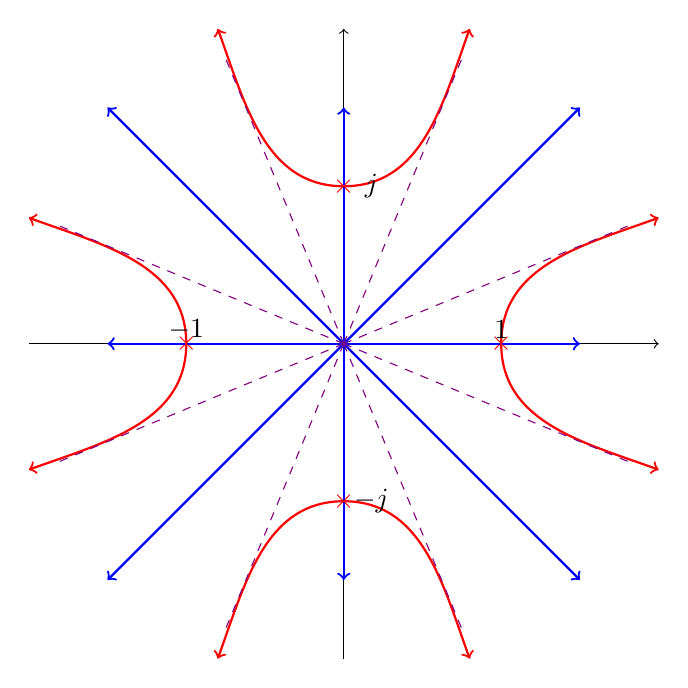
\begin{tikzpicture}[scale=2]
		\coordinate (o) at (0,0);
		\coordinate (ox) at (2,0);
   		\coordinate (oy) at (0,2);
		\draw[->] (-2,0) -- (ox);
		\draw[->] (0,-2) -- (oy);
		%\draw (o) node[below left] {$o$};
		\draw[thick,red] (-1,0) node {$\times$};
		\draw[thick,red] (1,0) node {$\times$};
		\draw[thick,red] (0,-1) node {$\times$};
		\draw[thick,red] (0,1) node {$\times$};
		
		\draw [<->,blue,thick] (-1.5,0)--(1.5,0);
   		\draw [<->,blue,thick] (0,-1.5)--(0,1.5);
   		\draw [<->,blue,thick] (-1.5,-1.5)--(1.5,1.5);
   		\draw [<->,blue,thick] (-1.5,1.5)--(1.5,-1.5);

		
		\draw [->,red,thick](-1,0) to [out=90,in=-20](-2,0.8);
		\draw [->,red,thick](-1,0) to [out=-90,in=20](-2,-0.8);
		\draw [->,red,thick](1,0) to [out=90,in=200](2,0.8);
		\draw [->,red,thick](1,0) to [out=-90,in=160](2,-0.8);

        \draw [->,red,thick](0,1) to [out=0,in=250](0.8,2);
		\draw [->,red,thick](0,1) to [out=180,in=-70](-0.8,2);
		\draw [->,red,thick](0,-1) to [out=0,in=110](0.8,-2);
		\draw [->,red,thick](0,-1) to [out=180,in=70](-0.8,-2);

		\draw [violet,dashed] (0,0)--+(22.5:2);
   		\draw [violet,dashed] (0,0)--+(67.5:2);
		\draw [violet,dashed] (0,0)--+(112.5:2);
		\draw [violet,dashed] (0,0)--+(157.5:2);
		\draw [violet,dashed] (0,0)--+(202.5:2);
		\draw [violet,dashed] (0,0)--+(247.5:2);
		\draw [violet,dashed] (0,0)--+(292.5:2);
		\draw [violet,dashed] (0,0)--+(337.5:2);

		%\draw (-1,0) node[below=1em] {$-1$};
		\draw (-1,0) node[xshift=0em ,yshift=0.5em] {$-1$};
		\draw (1,0) node[xshift=0em ,yshift=0.5em] {$1$};
		\draw (0,1) node[xshift=1em ,yshift=0em] {$j$};
		\draw (0,-1) node[xshift=1em ,yshift=0em] {$-j$};
		\end{tikzpicture}

}
}

\onlyanswer{\newpage}


\question(20分)已知单位负反馈系统开环传递函数:
$$G(s)=\frac{1}{s}\cdot e^{-s}$$
分析系统稳定性。若系统稳定,计算单位阶跃输入的稳态误差。

\onlyanswer
{
答:
\begin{align*}
G(j\omega)&=\frac{k}{j\omega}\cdot e^{j\omega}\\
\omega_c &= k \\
\omega_x &= \frac{\pi}{2}\\
\gamma  &=\frac{\pi}{2}-k
\end{align*}
$k<\frac{\pi}{2}$时,系统稳定,因此系统稳定。

由系统为I型系统可知,单位阶跃输入情况下稳态误差为0。

}



\question(20分)已知系统微分方程组如下:

\begin{align*}
\dot{y}(t) &=v(t) \\
\dot{v}(t) &=k_2\dot{r}(t)+r(t)-y(t)-k_1 v(t)
\end{align*}

绘制结构图;求解当 $v(0)=1,y(0)=1,r(t)=t$ 时的稳态误差;分析当$k_1,k_2$取何值时系统为临界阻尼系统。

\onlyanswer
{
答:

系统结构图如下:


\begin{tikzpicture}[scale=1, thick] 

\tikzstyle{block} = [draw,rectangle,thick,minimum height=1em,minimum width=1em]
\tikzstyle{sum} = [draw,circle,inner sep=0mm,minimum size=2mm]
\tikzstyle{branch} = [draw,circle,fill,inner sep=0pt,minimum size=0.5pt]
\tikzstyle{connector} = [->,thick]

\def\p(#1){\node[sum](p#1){};}
\def\b(#1){\node[branch](b#1){};}
\def\gr{\node[block](gr){ $k_2 s$ };}
\def\gk{\node[block](gk){ $k_1$ };}
\def\gh{\node[block](gh){$1$};}
\def\guv{\node[block](guv){$\dfrac{1}{ s}$};}
\def\gvy{\node[block](gvy){$\dfrac{1}{ s}$};}
\def\c{\node(c){$Y(s)$}; }
\def\r{\node(r){$R(s)$};}
\matrix[ampersand replacement=\&, row sep=1em, column sep=2em]{
	\&        \&   \gr    \\
	\r   \& \b(r) \&   \p(e)  \& \p(u)   \&\guv  \& \b(v)  \& \gvy    \& \b(y)  \&  \c\\
	\&         \&            \&          \& \gk\\
	\&         \&            \&           \& \gh\\
};

\draw [connector] (r) -- (pe);
\draw [connector] (br) |-(gr);
\draw [connector] (pe) -- node[midway,above] {$E(s)$}(pu);
\draw [connector] (gr) -|(pu);
\draw [connector] (pu) -- node[midway,above] {$U(s)$}(guv);
\draw [connector] (guv) -- node[midway,above] {$V(s)$}(gvy);
\draw [connector] (gvy) --(c);
\draw [connector]( bv) |-(gk);
\draw [connector] (gk) -| node[near end,left] {$-$} (pu);
\draw [connector] (by) |-(gh);
\draw [connector] (gh) -| node[very near end,left] {$-$} (pe);

\let\b\undefined
\let\p\donothing
\end{tikzpicture} 

考虑到初始条件,进行Laplace变换,得:
\begin{align*}
sY(s)-y(0) &=V(s) \\
sY(s)-1 &=V(s) \\
sV(s)-v(0) &=k_2 sR(s)+R(s)-Y(s)-k_1 V(s)\\
(s+k_1)V(s)-1 &=k_2 sR(s)+R(s)-Y(s)\\
s(s+k_1) Y(s)-(s+k_1)-1 &= k_2 sR(s)+R(s)-Y(s)\\
Y(s) &=\frac{k_2 sR(s)+R(s)+s+k_1+1}{s(s+k_1)+1}\\
E(s) &=R(s)-Y(s) \\
&=\frac{s(s+k_1)R(s)-k_2 sR(s)-s-k_1-1}{s(s+k_1)+1}
\end{align*}
当$k_1>0$时,系统稳定。当$k_1=2$时为临界阻尼系统。
$r(t)=t$时:
\begin{align*}
\lim_{s\to 0}sE(s) &=\frac{(s+k_1)-k_2 -s^2-k_1s-s}{s(s+k_1)+1}\\
&=k_1-k_2
\end{align*}
}


\question(20分)已知单位负反馈系统闭环传递函数:
	$$\Phi(s)=\frac{1}{s^3+3s^2+s+2}$$
分析系统稳定性与稳定裕度。


\onlyanswer
{
	答:
	Routh表:
$$
\begin{matrix}
 s^3  & 1 & 1 \\
 s^2  & 3 & 2 \\
 s^1  & \frac{1}{3}  & 0 \\
 s^0  & 2
\end{matrix}
$$
可知闭环系统稳定。

	系统开环传递函数为:
     $$G(s)=\frac{1}{s^3+3s^2+s+1}$$

计算相角裕度:
\begin{align*}
|G(j\omega_c)|&=1\\
\omega_c &=0\\
\gamma &=180^\circ
\end{align*}

原系统穿越频率$\omega_x$与开环传递函数为
$$G'(s)=\frac{k}{s^3+3s^2+s+1}$$
的系统相同。当选取合适的$k$使Nyquist曲线穿过(-1+0j)时,此时闭环系统
	$$\Phi'(s)=\frac{1}{s^3+3s^2+s+1+k}$$
存在纯虚根,可通过Routh判据计算出此时的$\omega_x$。

	Routh表:
	$$
	\begin{matrix}
	s^3  & 1 & 1 \\
	s^2  & 3 & 1+k \\
	s^1  & 1-\frac{1+k}{3} & 0 
	\end{matrix}
	$$
令$k=2$,则出现全零行,构建辅助方程$3s^2+3=0$,得:
\begin{align*}
\lambda &=\pm 1j \\
\omega_x &=1 \\
|G(j\omega_x )| &=\frac{1}{|-1j-3+1j+1|} \\
 &=\frac{1}{2} \\
h &= 2
\end{align*}


}
